\documentclass[twoside]{book}

% Packages required by doxygen
\usepackage{fixltx2e}
\usepackage{calc}
\usepackage{doxygen}
\usepackage[export]{adjustbox} % also loads graphicx
\usepackage{graphicx}
\usepackage[utf8]{inputenc}
\usepackage{makeidx}
\usepackage{multicol}
\usepackage{multirow}
\PassOptionsToPackage{warn}{textcomp}
\usepackage{textcomp}
\usepackage[nointegrals]{wasysym}
\usepackage[table]{xcolor}

% Font selection
\usepackage[T1]{fontenc}
\usepackage[scaled=.90]{helvet}
\usepackage{courier}
\usepackage{amssymb}
\usepackage{sectsty}
\renewcommand{\familydefault}{\sfdefault}
\allsectionsfont{%
  \fontseries{bc}\selectfont%
  \color{darkgray}%
}
\renewcommand{\DoxyLabelFont}{%
  \fontseries{bc}\selectfont%
  \color{darkgray}%
}
\newcommand{\+}{\discretionary{\mbox{\scriptsize$\hookleftarrow$}}{}{}}

% Page & text layout
\usepackage{geometry}
\geometry{%
  a4paper,%
  top=2.5cm,%
  bottom=2.5cm,%
  left=2.5cm,%
  right=2.5cm%
}
\tolerance=750
\hfuzz=15pt
\hbadness=750
\setlength{\emergencystretch}{15pt}
\setlength{\parindent}{0cm}
\setlength{\parskip}{3ex plus 2ex minus 2ex}
\makeatletter
\renewcommand{\paragraph}{%
  \@startsection{paragraph}{4}{0ex}{-1.0ex}{1.0ex}{%
    \normalfont\normalsize\bfseries\SS@parafont%
  }%
}
\renewcommand{\subparagraph}{%
  \@startsection{subparagraph}{5}{0ex}{-1.0ex}{1.0ex}{%
    \normalfont\normalsize\bfseries\SS@subparafont%
  }%
}
\makeatother

% Headers & footers
\usepackage{fancyhdr}
\pagestyle{fancyplain}
\fancyhead[LE]{\fancyplain{}{\bfseries\thepage}}
\fancyhead[CE]{\fancyplain{}{}}
\fancyhead[RE]{\fancyplain{}{\bfseries\leftmark}}
\fancyhead[LO]{\fancyplain{}{\bfseries\rightmark}}
\fancyhead[CO]{\fancyplain{}{}}
\fancyhead[RO]{\fancyplain{}{\bfseries\thepage}}
\fancyfoot[LE]{\fancyplain{}{}}
\fancyfoot[CE]{\fancyplain{}{}}
\fancyfoot[RE]{\fancyplain{}{\bfseries\scriptsize Generated by Doxygen }}
\fancyfoot[LO]{\fancyplain{}{\bfseries\scriptsize Generated by Doxygen }}
\fancyfoot[CO]{\fancyplain{}{}}
\fancyfoot[RO]{\fancyplain{}{}}
\renewcommand{\footrulewidth}{0.4pt}
\renewcommand{\chaptermark}[1]{%
  \markboth{#1}{}%
}
\renewcommand{\sectionmark}[1]{%
  \markright{\thesection\ #1}%
}

% Indices & bibliography
\usepackage{natbib}
\usepackage[titles]{tocloft}
\setcounter{tocdepth}{3}
\setcounter{secnumdepth}{5}
\makeindex

% Hyperlinks (required, but should be loaded last)
\usepackage{ifpdf}
\ifpdf
  \usepackage[pdftex,pagebackref=true]{hyperref}
\else
  \usepackage[ps2pdf,pagebackref=true]{hyperref}
\fi
\hypersetup{%
  colorlinks=true,%
  linkcolor=blue,%
  citecolor=blue,%
  unicode%
}

% Custom commands
\newcommand{\clearemptydoublepage}{%
  \newpage{\pagestyle{empty}\cleardoublepage}%
}

\usepackage{caption}
\captionsetup{labelsep=space,justification=centering,font={bf},singlelinecheck=off,skip=4pt,position=top}

%===== C O N T E N T S =====

\begin{document}

% Titlepage & ToC
\hypersetup{pageanchor=false,
             bookmarksnumbered=true,
             pdfencoding=unicode
            }
\pagenumbering{roman}
\begin{titlepage}
\vspace*{7cm}
\begin{center}%
{\Large I\+N\+E5418 Distributed Systems -\/ Mutual Exclusion Policy }\\
\vspace*{1cm}
{\large Generated by Doxygen 1.8.11}\\
\end{center}
\end{titlepage}
\clearemptydoublepage
\tableofcontents
\clearemptydoublepage
\pagenumbering{arabic}
\hypersetup{pageanchor=true}

%--- Begin generated contents ---
\chapter{Hierarchical Index}
\section{Class Hierarchy}
This inheritance list is sorted roughly, but not completely, alphabetically\+:\begin{DoxyCompactList}
\item \contentsline{section}{I\+PC}{\pageref{classdistributed__system_1_1IPC}}{}
\item \contentsline{section}{message\+\_\+t}{\pageref{structdistributed__system_1_1message__t}}{}
\item \contentsline{section}{Process}{\pageref{classdistributed__system_1_1Process}}{}
\begin{DoxyCompactList}
\item \contentsline{section}{Multicast\+Mutual\+Exclusion\+Policy}{\pageref{classdistributed__system_1_1MulticastMutualExclusionPolicy}}{}
\item \contentsline{section}{Server\+Mutual\+Exclusion\+Policy}{\pageref{classdistributed__system_1_1ServerMutualExclusionPolicy}}{}
\item \contentsline{section}{Token\+Ring\+Mutual\+Exclusion\+Policy}{\pageref{classdistributed__system_1_1TokenRingMutualExclusionPolicy}}{}
\end{DoxyCompactList}
\end{DoxyCompactList}

\chapter{Class Index}
\section{Class List}
Here are the classes, structs, unions and interfaces with brief descriptions\+:\begin{DoxyCompactList}
\item\contentsline{section}{\hyperlink{classdistributed__system_1_1IPC}{I\+PC} \\*Class that supports the user with the \hyperlink{classdistributed__system_1_1IPC}{I\+PC} A\+PI usage }{\pageref{classdistributed__system_1_1IPC}}{}
\item\contentsline{section}{\hyperlink{structdistributed__system_1_1message__t}{message\+\_\+t} }{\pageref{structdistributed__system_1_1message__t}}{}
\item\contentsline{section}{\hyperlink{classdistributed__system_1_1MulticastMutualExclusionPolicy}{Multicast\+Mutual\+Exclusion\+Policy} }{\pageref{classdistributed__system_1_1MulticastMutualExclusionPolicy}}{}
\item\contentsline{section}{\hyperlink{classdistributed__system_1_1Process}{Process} }{\pageref{classdistributed__system_1_1Process}}{}
\item\contentsline{section}{\hyperlink{classdistributed__system_1_1ServerMutualExclusionPolicy}{Server\+Mutual\+Exclusion\+Policy} }{\pageref{classdistributed__system_1_1ServerMutualExclusionPolicy}}{}
\item\contentsline{section}{\hyperlink{classdistributed__system_1_1TokenRingMutualExclusionPolicy}{Token\+Ring\+Mutual\+Exclusion\+Policy} }{\pageref{classdistributed__system_1_1TokenRingMutualExclusionPolicy}}{}
\end{DoxyCompactList}

\chapter{File Index}
\section{File List}
Here is a list of all documented files with brief descriptions\+:\begin{DoxyCompactList}
\item\contentsline{section}{include/{\bfseries const\+\_\+data.\+h} }{\pageref{const__data_8h}}{}
\item\contentsline{section}{include/\hyperlink{ipc_8h}{ipc.\+h} \\*High level approach to the low level I\+PC A\+PI }{\pageref{ipc_8h}}{}
\item\contentsline{section}{include/{\bfseries message.\+h} }{\pageref{message_8h}}{}
\item\contentsline{section}{include/{\bfseries multicast\+\_\+policy.\+h} }{\pageref{multicast__policy_8h}}{}
\item\contentsline{section}{include/{\bfseries process.\+h} }{\pageref{process_8h}}{}
\item\contentsline{section}{include/{\bfseries server\+\_\+policy.\+h} }{\pageref{server__policy_8h}}{}
\item\contentsline{section}{include/{\bfseries token\+\_\+ring\+\_\+policy.\+h} }{\pageref{token__ring__policy_8h}}{}
\item\contentsline{section}{src/\hyperlink{ipc_8cpp}{ipc.\+cpp} \\*High level approach to the low level I\+PC A\+PI }{\pageref{ipc_8cpp}}{}
\item\contentsline{section}{src/\hyperlink{main_8cpp}{main.\+cpp} \\*Main file responsible to read the arguments passed to the program, and start the process and the exclusion policy accordingly to it }{\pageref{main_8cpp}}{}
\item\contentsline{section}{src/{\bfseries multicast\+\_\+policy.\+cpp} }{\pageref{multicast__policy_8cpp}}{}
\item\contentsline{section}{src/{\bfseries process.\+cpp} }{\pageref{process_8cpp}}{}
\item\contentsline{section}{src/{\bfseries server\+\_\+policy.\+cpp} }{\pageref{server__policy_8cpp}}{}
\item\contentsline{section}{src/{\bfseries token\+\_\+ring\+\_\+policy.\+cpp} }{\pageref{token__ring__policy_8cpp}}{}
\end{DoxyCompactList}

\chapter{Class Documentation}
\hypertarget{classdistributed__system_1_1IPC}{}\section{I\+PC Class Reference}
\label{classdistributed__system_1_1IPC}\index{I\+PC@{I\+PC}}


Class that supports the user with the \hyperlink{classdistributed__system_1_1IPC}{I\+PC} A\+PI usage.  




{\ttfamily \#include \char`\"{}ipc.\+h\char`\"{}}

\subsection*{Public Member Functions}
\begin{DoxyCompactItemize}
\item 
\hyperlink{classdistributed__system_1_1IPC_a4f0157cf67601144761b69d6e4db15ef}{I\+PC} (int id)
\begin{DoxyCompactList}\small\item\em Constructor. \end{DoxyCompactList}\item 
void \hyperlink{classdistributed__system_1_1IPC_a02fd73d861ef2e4aabb38c0c9ff82947}{init} ()
\begin{DoxyCompactList}\small\item\em Call the file descriptor initialization. \end{DoxyCompactList}\item 
void {\bfseries start} ()\hypertarget{classdistributed__system_1_1IPC_a60de64d75454385b23995437f1d72669}{}\label{classdistributed__system_1_1IPC_a60de64d75454385b23995437f1d72669}

\item 
void \hyperlink{classdistributed__system_1_1IPC_a9cc1938afb0447727d7242cf37028fcb}{start\+\_\+listening} ()
\begin{DoxyCompactList}\small\item\em Start listening for other process messages. \end{DoxyCompactList}\item 
\hyperlink{structdistributed__system_1_1message__t}{message\+\_\+t} \hyperlink{classdistributed__system_1_1IPC_a16b7746dd0aedc9200f3253f4f3a9c36}{receive\+\_\+msg} ()
\begin{DoxyCompactList}\small\item\em Receive a message from other process. \end{DoxyCompactList}\item 
void \hyperlink{classdistributed__system_1_1IPC_acf64a1d5ddc831481592c0121f224b82}{send\+\_\+msg} (\hyperlink{structdistributed__system_1_1message__t}{message\+\_\+t})
\begin{DoxyCompactList}\small\item\em Send a message to another process. \end{DoxyCompactList}\end{DoxyCompactItemize}
\subsection*{Private Member Functions}
\begin{DoxyCompactItemize}
\item 
void \hyperlink{classdistributed__system_1_1IPC_adc5e10cc2794eaaf9cb71027024e564b}{create\+\_\+process\+\_\+fd} ()
\begin{DoxyCompactList}\small\item\em Create process socket file descriptor. \end{DoxyCompactList}\item 
void \hyperlink{classdistributed__system_1_1IPC_ac66af492ce97beaa2d384e584bcfed6a}{configure\+\_\+process\+\_\+fd} ()
\begin{DoxyCompactList}\small\item\em Configure process socket file descriptor. \end{DoxyCompactList}\end{DoxyCompactItemize}
\subsection*{Private Attributes}
\begin{DoxyCompactItemize}
\item 
int \hyperlink{classdistributed__system_1_1IPC_aafd0c2f55b73e7a1d4bd1174fdebbcf8}{id\+\_\+}
\begin{DoxyCompactList}\small\item\em \hyperlink{classdistributed__system_1_1Process}{Process} id attached to this \hyperlink{classdistributed__system_1_1IPC}{I\+PC}. \end{DoxyCompactList}\item 
int \hyperlink{classdistributed__system_1_1IPC_a7f99d156ebf648d3ff1c3f1db1b84e99}{opt\+\_\+}
\begin{DoxyCompactList}\small\item\em Always 1, relative to socket operation. \end{DoxyCompactList}\item 
int \hyperlink{classdistributed__system_1_1IPC_a92e821fba37e04797ca9ef2c29490e37}{rcv\+\_\+process\+\_\+fd\+\_\+}
\begin{DoxyCompactList}\small\item\em File descriptor, to received messages. \end{DoxyCompactList}\item 
int \hyperlink{classdistributed__system_1_1IPC_acd0d035f1eb6ec4e35eb6adb1a4ebd8c}{send\+\_\+process\+\_\+fd\+\_\+}
\begin{DoxyCompactList}\small\item\em File descriptor, to send messages. \end{DoxyCompactList}\item 
int \hyperlink{classdistributed__system_1_1IPC_ac9d328f95fad3be2cd1b2aa3bfbe0e9d}{address\+\_\+length\+\_\+}
\begin{DoxyCompactList}\small\item\em Length of the address. \end{DoxyCompactList}\item 
int \hyperlink{classdistributed__system_1_1IPC_adffbfa5995d32588eb323ce4c684fae7}{socket\+\_\+port\+\_\+}
\begin{DoxyCompactList}\small\item\em Socket port that \hyperlink{classdistributed__system_1_1Process}{Process} will be bind. \end{DoxyCompactList}\item 
struct sockaddr\+\_\+in \hyperlink{classdistributed__system_1_1IPC_a051ae791ace72a56982febd4267912a0}{address\+\_\+}
\begin{DoxyCompactList}\small\item\em Struct responsible to configure sockets. \end{DoxyCompactList}\end{DoxyCompactItemize}


\subsection{Detailed Description}
Class that supports the user with the \hyperlink{classdistributed__system_1_1IPC}{I\+PC} A\+PI usage. 

Definition at line 25 of file ipc.\+h.



\subsection{Constructor \& Destructor Documentation}
\index{distributed\+\_\+system\+::\+I\+PC@{distributed\+\_\+system\+::\+I\+PC}!I\+PC@{I\+PC}}
\index{I\+PC@{I\+PC}!distributed\+\_\+system\+::\+I\+PC@{distributed\+\_\+system\+::\+I\+PC}}
\subsubsection[{\texorpdfstring{I\+P\+C(int id)}{IPC(int id)}}]{\setlength{\rightskip}{0pt plus 5cm}{\bf I\+PC} (
\begin{DoxyParamCaption}
\item[{int}]{id}
\end{DoxyParamCaption}
)}\hypertarget{classdistributed__system_1_1IPC_a4f0157cf67601144761b69d6e4db15ef}{}\label{classdistributed__system_1_1IPC_a4f0157cf67601144761b69d6e4db15ef}


Constructor. 

Set initial attributes values.


\begin{DoxyParams}{Parameters}
{\em id} & the id of the process that this \hyperlink{classdistributed__system_1_1IPC}{I\+PC} will be responsible for. \\
\hline
\end{DoxyParams}


Definition at line 30 of file ipc.\+cpp.



\subsection{Member Function Documentation}
\index{distributed\+\_\+system\+::\+I\+PC@{distributed\+\_\+system\+::\+I\+PC}!configure\+\_\+process\+\_\+fd@{configure\+\_\+process\+\_\+fd}}
\index{configure\+\_\+process\+\_\+fd@{configure\+\_\+process\+\_\+fd}!distributed\+\_\+system\+::\+I\+PC@{distributed\+\_\+system\+::\+I\+PC}}
\subsubsection[{\texorpdfstring{configure\+\_\+process\+\_\+fd()}{configure_process_fd()}}]{\setlength{\rightskip}{0pt plus 5cm}void configure\+\_\+process\+\_\+fd (
\begin{DoxyParamCaption}
{}
\end{DoxyParamCaption}
)\hspace{0.3cm}{\ttfamily [private]}}\hypertarget{classdistributed__system_1_1IPC_ac66af492ce97beaa2d384e584bcfed6a}{}\label{classdistributed__system_1_1IPC_ac66af492ce97beaa2d384e584bcfed6a}


Configure process socket file descriptor. 



Definition at line 58 of file ipc.\+cpp.

\index{distributed\+\_\+system\+::\+I\+PC@{distributed\+\_\+system\+::\+I\+PC}!create\+\_\+process\+\_\+fd@{create\+\_\+process\+\_\+fd}}
\index{create\+\_\+process\+\_\+fd@{create\+\_\+process\+\_\+fd}!distributed\+\_\+system\+::\+I\+PC@{distributed\+\_\+system\+::\+I\+PC}}
\subsubsection[{\texorpdfstring{create\+\_\+process\+\_\+fd()}{create_process_fd()}}]{\setlength{\rightskip}{0pt plus 5cm}void create\+\_\+process\+\_\+fd (
\begin{DoxyParamCaption}
{}
\end{DoxyParamCaption}
)\hspace{0.3cm}{\ttfamily [private]}}\hypertarget{classdistributed__system_1_1IPC_adc5e10cc2794eaaf9cb71027024e564b}{}\label{classdistributed__system_1_1IPC_adc5e10cc2794eaaf9cb71027024e564b}


Create process socket file descriptor. 



Definition at line 46 of file ipc.\+cpp.

\index{distributed\+\_\+system\+::\+I\+PC@{distributed\+\_\+system\+::\+I\+PC}!init@{init}}
\index{init@{init}!distributed\+\_\+system\+::\+I\+PC@{distributed\+\_\+system\+::\+I\+PC}}
\subsubsection[{\texorpdfstring{init()}{init()}}]{\setlength{\rightskip}{0pt plus 5cm}void init (
\begin{DoxyParamCaption}
{}
\end{DoxyParamCaption}
)}\hypertarget{classdistributed__system_1_1IPC_a02fd73d861ef2e4aabb38c0c9ff82947}{}\label{classdistributed__system_1_1IPC_a02fd73d861ef2e4aabb38c0c9ff82947}


Call the file descriptor initialization. 



Definition at line 37 of file ipc.\+cpp.

\index{distributed\+\_\+system\+::\+I\+PC@{distributed\+\_\+system\+::\+I\+PC}!receive\+\_\+msg@{receive\+\_\+msg}}
\index{receive\+\_\+msg@{receive\+\_\+msg}!distributed\+\_\+system\+::\+I\+PC@{distributed\+\_\+system\+::\+I\+PC}}
\subsubsection[{\texorpdfstring{receive\+\_\+msg()}{receive_msg()}}]{\setlength{\rightskip}{0pt plus 5cm}{\bf message\+\_\+t} receive\+\_\+msg (
\begin{DoxyParamCaption}
{}
\end{DoxyParamCaption}
)}\hypertarget{classdistributed__system_1_1IPC_a16b7746dd0aedc9200f3253f4f3a9c36}{}\label{classdistributed__system_1_1IPC_a16b7746dd0aedc9200f3253f4f3a9c36}


Receive a message from other process. 

\begin{DoxyReturn}{Returns}
the received message. 
\end{DoxyReturn}


Definition at line 98 of file ipc.\+cpp.

\index{distributed\+\_\+system\+::\+I\+PC@{distributed\+\_\+system\+::\+I\+PC}!send\+\_\+msg@{send\+\_\+msg}}
\index{send\+\_\+msg@{send\+\_\+msg}!distributed\+\_\+system\+::\+I\+PC@{distributed\+\_\+system\+::\+I\+PC}}
\subsubsection[{\texorpdfstring{send\+\_\+msg(message\+\_\+t)}{send_msg(message_t)}}]{\setlength{\rightskip}{0pt plus 5cm}void send\+\_\+msg (
\begin{DoxyParamCaption}
\item[{{\bf message\+\_\+t}}]{msg}
\end{DoxyParamCaption}
)}\hypertarget{classdistributed__system_1_1IPC_acf64a1d5ddc831481592c0121f224b82}{}\label{classdistributed__system_1_1IPC_acf64a1d5ddc831481592c0121f224b82}


Send a message to another process. 


\begin{DoxyParams}{Parameters}
{\em msg} & message to be sent. \\
\hline
\end{DoxyParams}


Definition at line 126 of file ipc.\+cpp.

\index{distributed\+\_\+system\+::\+I\+PC@{distributed\+\_\+system\+::\+I\+PC}!start\+\_\+listening@{start\+\_\+listening}}
\index{start\+\_\+listening@{start\+\_\+listening}!distributed\+\_\+system\+::\+I\+PC@{distributed\+\_\+system\+::\+I\+PC}}
\subsubsection[{\texorpdfstring{start\+\_\+listening()}{start_listening()}}]{\setlength{\rightskip}{0pt plus 5cm}void start\+\_\+listening (
\begin{DoxyParamCaption}
{}
\end{DoxyParamCaption}
)}\hypertarget{classdistributed__system_1_1IPC_a9cc1938afb0447727d7242cf37028fcb}{}\label{classdistributed__system_1_1IPC_a9cc1938afb0447727d7242cf37028fcb}


Start listening for other process messages. 



Definition at line 84 of file ipc.\+cpp.



\subsection{Member Data Documentation}
\index{distributed\+\_\+system\+::\+I\+PC@{distributed\+\_\+system\+::\+I\+PC}!address\+\_\+@{address\+\_\+}}
\index{address\+\_\+@{address\+\_\+}!distributed\+\_\+system\+::\+I\+PC@{distributed\+\_\+system\+::\+I\+PC}}
\subsubsection[{\texorpdfstring{address\+\_\+}{address_}}]{\setlength{\rightskip}{0pt plus 5cm}struct sockaddr\+\_\+in address\+\_\+\hspace{0.3cm}{\ttfamily [private]}}\hypertarget{classdistributed__system_1_1IPC_a051ae791ace72a56982febd4267912a0}{}\label{classdistributed__system_1_1IPC_a051ae791ace72a56982febd4267912a0}


Struct responsible to configure sockets. 



Definition at line 45 of file ipc.\+h.

\index{distributed\+\_\+system\+::\+I\+PC@{distributed\+\_\+system\+::\+I\+PC}!address\+\_\+length\+\_\+@{address\+\_\+length\+\_\+}}
\index{address\+\_\+length\+\_\+@{address\+\_\+length\+\_\+}!distributed\+\_\+system\+::\+I\+PC@{distributed\+\_\+system\+::\+I\+PC}}
\subsubsection[{\texorpdfstring{address\+\_\+length\+\_\+}{address_length_}}]{\setlength{\rightskip}{0pt plus 5cm}int address\+\_\+length\+\_\+\hspace{0.3cm}{\ttfamily [private]}}\hypertarget{classdistributed__system_1_1IPC_ac9d328f95fad3be2cd1b2aa3bfbe0e9d}{}\label{classdistributed__system_1_1IPC_ac9d328f95fad3be2cd1b2aa3bfbe0e9d}


Length of the address. 



Definition at line 43 of file ipc.\+h.

\index{distributed\+\_\+system\+::\+I\+PC@{distributed\+\_\+system\+::\+I\+PC}!id\+\_\+@{id\+\_\+}}
\index{id\+\_\+@{id\+\_\+}!distributed\+\_\+system\+::\+I\+PC@{distributed\+\_\+system\+::\+I\+PC}}
\subsubsection[{\texorpdfstring{id\+\_\+}{id_}}]{\setlength{\rightskip}{0pt plus 5cm}int id\+\_\+\hspace{0.3cm}{\ttfamily [private]}}\hypertarget{classdistributed__system_1_1IPC_aafd0c2f55b73e7a1d4bd1174fdebbcf8}{}\label{classdistributed__system_1_1IPC_aafd0c2f55b73e7a1d4bd1174fdebbcf8}


\hyperlink{classdistributed__system_1_1Process}{Process} id attached to this \hyperlink{classdistributed__system_1_1IPC}{I\+PC}. 



Definition at line 39 of file ipc.\+h.

\index{distributed\+\_\+system\+::\+I\+PC@{distributed\+\_\+system\+::\+I\+PC}!opt\+\_\+@{opt\+\_\+}}
\index{opt\+\_\+@{opt\+\_\+}!distributed\+\_\+system\+::\+I\+PC@{distributed\+\_\+system\+::\+I\+PC}}
\subsubsection[{\texorpdfstring{opt\+\_\+}{opt_}}]{\setlength{\rightskip}{0pt plus 5cm}int opt\+\_\+\hspace{0.3cm}{\ttfamily [private]}}\hypertarget{classdistributed__system_1_1IPC_a7f99d156ebf648d3ff1c3f1db1b84e99}{}\label{classdistributed__system_1_1IPC_a7f99d156ebf648d3ff1c3f1db1b84e99}


Always 1, relative to socket operation. 



Definition at line 40 of file ipc.\+h.

\index{distributed\+\_\+system\+::\+I\+PC@{distributed\+\_\+system\+::\+I\+PC}!rcv\+\_\+process\+\_\+fd\+\_\+@{rcv\+\_\+process\+\_\+fd\+\_\+}}
\index{rcv\+\_\+process\+\_\+fd\+\_\+@{rcv\+\_\+process\+\_\+fd\+\_\+}!distributed\+\_\+system\+::\+I\+PC@{distributed\+\_\+system\+::\+I\+PC}}
\subsubsection[{\texorpdfstring{rcv\+\_\+process\+\_\+fd\+\_\+}{rcv_process_fd_}}]{\setlength{\rightskip}{0pt plus 5cm}int rcv\+\_\+process\+\_\+fd\+\_\+\hspace{0.3cm}{\ttfamily [private]}}\hypertarget{classdistributed__system_1_1IPC_a92e821fba37e04797ca9ef2c29490e37}{}\label{classdistributed__system_1_1IPC_a92e821fba37e04797ca9ef2c29490e37}


File descriptor, to received messages. 



Definition at line 41 of file ipc.\+h.

\index{distributed\+\_\+system\+::\+I\+PC@{distributed\+\_\+system\+::\+I\+PC}!send\+\_\+process\+\_\+fd\+\_\+@{send\+\_\+process\+\_\+fd\+\_\+}}
\index{send\+\_\+process\+\_\+fd\+\_\+@{send\+\_\+process\+\_\+fd\+\_\+}!distributed\+\_\+system\+::\+I\+PC@{distributed\+\_\+system\+::\+I\+PC}}
\subsubsection[{\texorpdfstring{send\+\_\+process\+\_\+fd\+\_\+}{send_process_fd_}}]{\setlength{\rightskip}{0pt plus 5cm}int send\+\_\+process\+\_\+fd\+\_\+\hspace{0.3cm}{\ttfamily [private]}}\hypertarget{classdistributed__system_1_1IPC_acd0d035f1eb6ec4e35eb6adb1a4ebd8c}{}\label{classdistributed__system_1_1IPC_acd0d035f1eb6ec4e35eb6adb1a4ebd8c}


File descriptor, to send messages. 



Definition at line 42 of file ipc.\+h.

\index{distributed\+\_\+system\+::\+I\+PC@{distributed\+\_\+system\+::\+I\+PC}!socket\+\_\+port\+\_\+@{socket\+\_\+port\+\_\+}}
\index{socket\+\_\+port\+\_\+@{socket\+\_\+port\+\_\+}!distributed\+\_\+system\+::\+I\+PC@{distributed\+\_\+system\+::\+I\+PC}}
\subsubsection[{\texorpdfstring{socket\+\_\+port\+\_\+}{socket_port_}}]{\setlength{\rightskip}{0pt plus 5cm}int socket\+\_\+port\+\_\+\hspace{0.3cm}{\ttfamily [private]}}\hypertarget{classdistributed__system_1_1IPC_adffbfa5995d32588eb323ce4c684fae7}{}\label{classdistributed__system_1_1IPC_adffbfa5995d32588eb323ce4c684fae7}


Socket port that \hyperlink{classdistributed__system_1_1Process}{Process} will be bind. 



Definition at line 44 of file ipc.\+h.



The documentation for this class was generated from the following files\+:\begin{DoxyCompactItemize}
\item 
include/\hyperlink{ipc_8h}{ipc.\+h}\item 
src/\hyperlink{ipc_8cpp}{ipc.\+cpp}\end{DoxyCompactItemize}

\hypertarget{structdistributed__system_1_1message__t}{}\section{message\+\_\+t Struct Reference}
\label{structdistributed__system_1_1message__t}\index{message\+\_\+t@{message\+\_\+t}}
\subsection*{Public Attributes}
\begin{DoxyCompactItemize}
\item 
char {\bfseries source} \mbox{[}4\mbox{]}\hypertarget{structdistributed__system_1_1message__t_aa3c7a4db993a2d188f67be9552a1ba9d}{}\label{structdistributed__system_1_1message__t_aa3c7a4db993a2d188f67be9552a1ba9d}

\item 
char {\bfseries destination} \mbox{[}4\mbox{]}\hypertarget{structdistributed__system_1_1message__t_ad51f70831a1d09a124fd6556c5f2f6f3}{}\label{structdistributed__system_1_1message__t_ad51f70831a1d09a124fd6556c5f2f6f3}

\item 
char {\bfseries type} \mbox{[}4\mbox{]}\hypertarget{structdistributed__system_1_1message__t_a4083c19bc4225336c3fd9e00d40ee18e}{}\label{structdistributed__system_1_1message__t_a4083c19bc4225336c3fd9e00d40ee18e}

\item 
char {\bfseries data} \mbox{[}100\mbox{]}\hypertarget{structdistributed__system_1_1message__t_a351608c09e54a0c2e6ea1f551146e348}{}\label{structdistributed__system_1_1message__t_a351608c09e54a0c2e6ea1f551146e348}

\end{DoxyCompactItemize}


\subsection{Detailed Description}


Definition at line 12 of file message.\+h.



The documentation for this struct was generated from the following file\+:\begin{DoxyCompactItemize}
\item 
include/message.\+h\end{DoxyCompactItemize}

\hypertarget{classdistributed__system_1_1MulticastMutualExclusionPolicy}{}\section{Multicast\+Mutual\+Exclusion\+Policy Class Reference}
\label{classdistributed__system_1_1MulticastMutualExclusionPolicy}\index{Multicast\+Mutual\+Exclusion\+Policy@{Multicast\+Mutual\+Exclusion\+Policy}}
Inheritance diagram for Multicast\+Mutual\+Exclusion\+Policy\+:\begin{figure}[H]
\begin{center}
\leavevmode
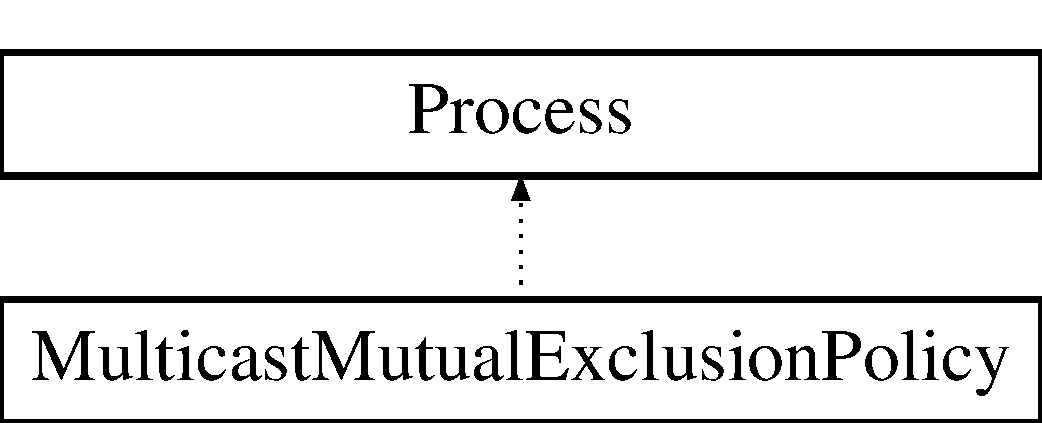
\includegraphics[height=2.000000cm]{classdistributed__system_1_1MulticastMutualExclusionPolicy}
\end{center}
\end{figure}
\subsection*{Public Member Functions}
\begin{DoxyCompactItemize}
\item 
{\bfseries Multicast\+Mutual\+Exclusion\+Policy} (int id, int n\+\_\+process)\hypertarget{classdistributed__system_1_1MulticastMutualExclusionPolicy_aec982e06c8b0794c5c65301c59db568f}{}\label{classdistributed__system_1_1MulticastMutualExclusionPolicy_aec982e06c8b0794c5c65301c59db568f}

\item 
void {\bfseries run} ()\hypertarget{classdistributed__system_1_1MulticastMutualExclusionPolicy_a13a43e6d814de94978c515cb084873b1}{}\label{classdistributed__system_1_1MulticastMutualExclusionPolicy_a13a43e6d814de94978c515cb084873b1}

\end{DoxyCompactItemize}
\subsection*{Private Member Functions}
\begin{DoxyCompactItemize}
\item 
void {\bfseries process\+\_\+message} ()\hypertarget{classdistributed__system_1_1MulticastMutualExclusionPolicy_aaaa542ed11f0470f15a18b01754e7058}{}\label{classdistributed__system_1_1MulticastMutualExclusionPolicy_aaaa542ed11f0470f15a18b01754e7058}

\item 
int {\bfseries destination} ()\hypertarget{classdistributed__system_1_1MulticastMutualExclusionPolicy_a427480a43d844be55be63f111d8805dd}{}\label{classdistributed__system_1_1MulticastMutualExclusionPolicy_a427480a43d844be55be63f111d8805dd}

\item 
void {\bfseries send\+\_\+token} ()\hypertarget{classdistributed__system_1_1MulticastMutualExclusionPolicy_af48d2022be2f51f240ef71f4108adbd7}{}\label{classdistributed__system_1_1MulticastMutualExclusionPolicy_af48d2022be2f51f240ef71f4108adbd7}

\item 
void {\bfseries server\+\_\+resource\+\_\+request} ()\hypertarget{classdistributed__system_1_1MulticastMutualExclusionPolicy_af42000fbadb1729fbd6a7e357dcae6ca}{}\label{classdistributed__system_1_1MulticastMutualExclusionPolicy_af42000fbadb1729fbd6a7e357dcae6ca}

\item 
void {\bfseries server\+\_\+resource\+\_\+release} ()\hypertarget{classdistributed__system_1_1MulticastMutualExclusionPolicy_ad63c50cc4e3443242e9c30636ec51b0c}{}\label{classdistributed__system_1_1MulticastMutualExclusionPolicy_ad63c50cc4e3443242e9c30636ec51b0c}

\item 
void {\bfseries client\+\_\+resource\+\_\+request} ()\hypertarget{classdistributed__system_1_1MulticastMutualExclusionPolicy_a24ee654e617f14425f0fedb837bdad6c}{}\label{classdistributed__system_1_1MulticastMutualExclusionPolicy_a24ee654e617f14425f0fedb837bdad6c}

\item 
void {\bfseries client\+\_\+resource\+\_\+release} ()\hypertarget{classdistributed__system_1_1MulticastMutualExclusionPolicy_a22143366b590cd8072c99e4942fcded2}{}\label{classdistributed__system_1_1MulticastMutualExclusionPolicy_a22143366b590cd8072c99e4942fcded2}

\item 
void {\bfseries start\+\_\+broadcast} ()\hypertarget{classdistributed__system_1_1MulticastMutualExclusionPolicy_a71d593aee31d2ec47bf9c5d7ed97bfdd}{}\label{classdistributed__system_1_1MulticastMutualExclusionPolicy_a71d593aee31d2ec47bf9c5d7ed97bfdd}

\end{DoxyCompactItemize}
\subsection*{Private Attributes}
\begin{DoxyCompactItemize}
\item 
std\+::queue$<$ int $>$ {\bfseries work\+\_\+queue}\hypertarget{classdistributed__system_1_1MulticastMutualExclusionPolicy_a3b83f6d4011132a21b274e445d36b740}{}\label{classdistributed__system_1_1MulticastMutualExclusionPolicy_a3b83f6d4011132a21b274e445d36b740}

\end{DoxyCompactItemize}


\subsection{Detailed Description}


Definition at line 9 of file multicast\+\_\+policy.\+h.



The documentation for this class was generated from the following files\+:\begin{DoxyCompactItemize}
\item 
include/multicast\+\_\+policy.\+h\item 
src/multicast\+\_\+policy.\+cpp\end{DoxyCompactItemize}

\hypertarget{classdistributed__system_1_1Process}{}\section{Process Class Reference}
\label{classdistributed__system_1_1Process}\index{Process@{Process}}
Inheritance diagram for Process\+:\begin{figure}[H]
\begin{center}
\leavevmode
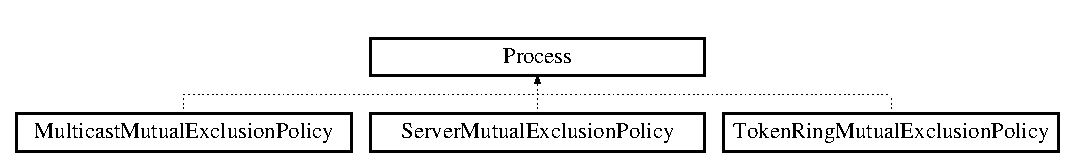
\includegraphics[height=1.812298cm]{classdistributed__system_1_1Process}
\end{center}
\end{figure}
\subsection*{Public Member Functions}
\begin{DoxyCompactItemize}
\item 
{\bfseries Process} (int id, int n\+\_\+process)\hypertarget{classdistributed__system_1_1Process_a38d5653c5327038426dd69393130c775}{}\label{classdistributed__system_1_1Process_a38d5653c5327038426dd69393130c775}

\end{DoxyCompactItemize}
\subsection*{Protected Member Functions}
\begin{DoxyCompactItemize}
\item 
void {\bfseries compute} ()\hypertarget{classdistributed__system_1_1Process_a4993c97a669fa259c6574a18d547c117}{}\label{classdistributed__system_1_1Process_a4993c97a669fa259c6574a18d547c117}

\item 
int {\bfseries random\+\_\+computation\+\_\+time} ()\hypertarget{classdistributed__system_1_1Process_ab9067ec75c01e0143a81b0c4d7fe5d6b}{}\label{classdistributed__system_1_1Process_ab9067ec75c01e0143a81b0c4d7fe5d6b}

\end{DoxyCompactItemize}
\subsection*{Protected Attributes}
\begin{DoxyCompactItemize}
\item 
int {\bfseries id\+\_\+}\hypertarget{classdistributed__system_1_1Process_aafd0c2f55b73e7a1d4bd1174fdebbcf8}{}\label{classdistributed__system_1_1Process_aafd0c2f55b73e7a1d4bd1174fdebbcf8}

\item 
int {\bfseries n\+\_\+process\+\_\+}\hypertarget{classdistributed__system_1_1Process_a289b1e6562f8fb42908a202b2f6485ff}{}\label{classdistributed__system_1_1Process_a289b1e6562f8fb42908a202b2f6485ff}

\item 
int {\bfseries computation\+\_\+time\+\_\+}\hypertarget{classdistributed__system_1_1Process_a6240cc652eb1f42271c5d259e468449e}{}\label{classdistributed__system_1_1Process_a6240cc652eb1f42271c5d259e468449e}

\item 
\hyperlink{classdistributed__system_1_1IPC}{I\+PC} {\bfseries ipc\+\_\+}\hypertarget{classdistributed__system_1_1Process_a2b91c717adb1a58d751fbce17f19d50a}{}\label{classdistributed__system_1_1Process_a2b91c717adb1a58d751fbce17f19d50a}

\item 
\hyperlink{structdistributed__system_1_1message__t}{message\+\_\+t} {\bfseries received\+\_\+message\+\_\+}\hypertarget{classdistributed__system_1_1Process_a08cdc7cdd554e995921af2430e00eece}{}\label{classdistributed__system_1_1Process_a08cdc7cdd554e995921af2430e00eece}

\end{DoxyCompactItemize}


\subsection{Detailed Description}


Definition at line 9 of file process.\+h.



The documentation for this class was generated from the following files\+:\begin{DoxyCompactItemize}
\item 
include/process.\+h\item 
src/process.\+cpp\end{DoxyCompactItemize}

\hypertarget{classdistributed__system_1_1ServerMutualExclusionPolicy}{}\section{Server\+Mutual\+Exclusion\+Policy Class Reference}
\label{classdistributed__system_1_1ServerMutualExclusionPolicy}\index{Server\+Mutual\+Exclusion\+Policy@{Server\+Mutual\+Exclusion\+Policy}}
Inheritance diagram for Server\+Mutual\+Exclusion\+Policy\+:\begin{figure}[H]
\begin{center}
\leavevmode
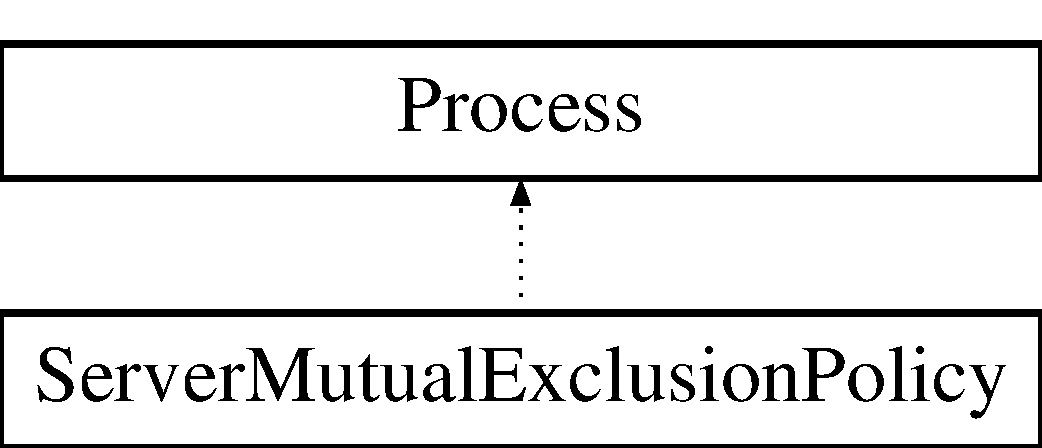
\includegraphics[height=2.000000cm]{classdistributed__system_1_1ServerMutualExclusionPolicy}
\end{center}
\end{figure}
\subsection*{Public Member Functions}
\begin{DoxyCompactItemize}
\item 
{\bfseries Server\+Mutual\+Exclusion\+Policy} (int id, int n\+\_\+process)\hypertarget{classdistributed__system_1_1ServerMutualExclusionPolicy_ac92be0175c62808b6cc40992a7a18b45}{}\label{classdistributed__system_1_1ServerMutualExclusionPolicy_ac92be0175c62808b6cc40992a7a18b45}

\item 
void {\bfseries run} ()\hypertarget{classdistributed__system_1_1ServerMutualExclusionPolicy_a13a43e6d814de94978c515cb084873b1}{}\label{classdistributed__system_1_1ServerMutualExclusionPolicy_a13a43e6d814de94978c515cb084873b1}

\end{DoxyCompactItemize}
\subsection*{Private Member Functions}
\begin{DoxyCompactItemize}
\item 
void {\bfseries process\+\_\+message} ()\hypertarget{classdistributed__system_1_1ServerMutualExclusionPolicy_aaaa542ed11f0470f15a18b01754e7058}{}\label{classdistributed__system_1_1ServerMutualExclusionPolicy_aaaa542ed11f0470f15a18b01754e7058}

\item 
int {\bfseries destination} ()\hypertarget{classdistributed__system_1_1ServerMutualExclusionPolicy_a427480a43d844be55be63f111d8805dd}{}\label{classdistributed__system_1_1ServerMutualExclusionPolicy_a427480a43d844be55be63f111d8805dd}

\item 
void {\bfseries send\+\_\+token} ()\hypertarget{classdistributed__system_1_1ServerMutualExclusionPolicy_af48d2022be2f51f240ef71f4108adbd7}{}\label{classdistributed__system_1_1ServerMutualExclusionPolicy_af48d2022be2f51f240ef71f4108adbd7}

\item 
void {\bfseries server\+\_\+resource\+\_\+request} ()\hypertarget{classdistributed__system_1_1ServerMutualExclusionPolicy_af42000fbadb1729fbd6a7e357dcae6ca}{}\label{classdistributed__system_1_1ServerMutualExclusionPolicy_af42000fbadb1729fbd6a7e357dcae6ca}

\item 
void {\bfseries server\+\_\+resource\+\_\+release} ()\hypertarget{classdistributed__system_1_1ServerMutualExclusionPolicy_ad63c50cc4e3443242e9c30636ec51b0c}{}\label{classdistributed__system_1_1ServerMutualExclusionPolicy_ad63c50cc4e3443242e9c30636ec51b0c}

\item 
void {\bfseries client\+\_\+resource\+\_\+request} ()\hypertarget{classdistributed__system_1_1ServerMutualExclusionPolicy_a24ee654e617f14425f0fedb837bdad6c}{}\label{classdistributed__system_1_1ServerMutualExclusionPolicy_a24ee654e617f14425f0fedb837bdad6c}

\item 
void {\bfseries client\+\_\+resource\+\_\+release} ()\hypertarget{classdistributed__system_1_1ServerMutualExclusionPolicy_a22143366b590cd8072c99e4942fcded2}{}\label{classdistributed__system_1_1ServerMutualExclusionPolicy_a22143366b590cd8072c99e4942fcded2}

\item 
void {\bfseries start\+\_\+broadcast} ()\hypertarget{classdistributed__system_1_1ServerMutualExclusionPolicy_a71d593aee31d2ec47bf9c5d7ed97bfdd}{}\label{classdistributed__system_1_1ServerMutualExclusionPolicy_a71d593aee31d2ec47bf9c5d7ed97bfdd}

\end{DoxyCompactItemize}
\subsection*{Private Attributes}
\begin{DoxyCompactItemize}
\item 
std\+::queue$<$ int $>$ {\bfseries work\+\_\+queue}\hypertarget{classdistributed__system_1_1ServerMutualExclusionPolicy_a3b83f6d4011132a21b274e445d36b740}{}\label{classdistributed__system_1_1ServerMutualExclusionPolicy_a3b83f6d4011132a21b274e445d36b740}

\end{DoxyCompactItemize}


\subsection{Detailed Description}


Definition at line 9 of file server\+\_\+policy.\+h.



The documentation for this class was generated from the following files\+:\begin{DoxyCompactItemize}
\item 
include/server\+\_\+policy.\+h\item 
src/server\+\_\+policy.\+cpp\end{DoxyCompactItemize}

\hypertarget{classdistributed__system_1_1TokenRingMutualExclusionPolicy}{}\section{Token\+Ring\+Mutual\+Exclusion\+Policy Class Reference}
\label{classdistributed__system_1_1TokenRingMutualExclusionPolicy}\index{Token\+Ring\+Mutual\+Exclusion\+Policy@{Token\+Ring\+Mutual\+Exclusion\+Policy}}
Inheritance diagram for Token\+Ring\+Mutual\+Exclusion\+Policy\+:\begin{figure}[H]
\begin{center}
\leavevmode
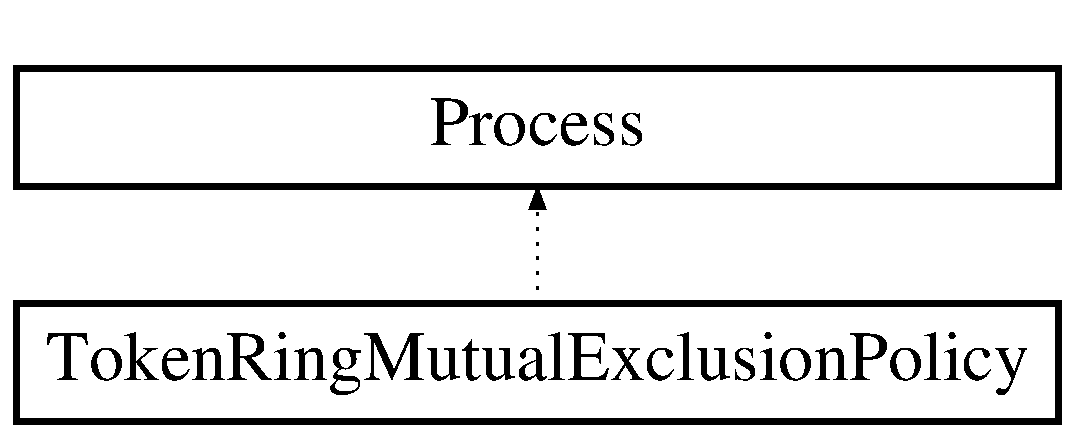
\includegraphics[height=2.000000cm]{classdistributed__system_1_1TokenRingMutualExclusionPolicy}
\end{center}
\end{figure}
\subsection*{Public Member Functions}
\begin{DoxyCompactItemize}
\item 
{\bfseries Token\+Ring\+Mutual\+Exclusion\+Policy} (int id, int n\+\_\+process)\hypertarget{classdistributed__system_1_1TokenRingMutualExclusionPolicy_ae1bc7fad7c29f21626a46e7a587330e3}{}\label{classdistributed__system_1_1TokenRingMutualExclusionPolicy_ae1bc7fad7c29f21626a46e7a587330e3}

\item 
void {\bfseries run} ()\hypertarget{classdistributed__system_1_1TokenRingMutualExclusionPolicy_a13a43e6d814de94978c515cb084873b1}{}\label{classdistributed__system_1_1TokenRingMutualExclusionPolicy_a13a43e6d814de94978c515cb084873b1}

\end{DoxyCompactItemize}
\subsection*{Private Member Functions}
\begin{DoxyCompactItemize}
\item 
void {\bfseries process\+\_\+message} ()\hypertarget{classdistributed__system_1_1TokenRingMutualExclusionPolicy_aaaa542ed11f0470f15a18b01754e7058}{}\label{classdistributed__system_1_1TokenRingMutualExclusionPolicy_aaaa542ed11f0470f15a18b01754e7058}

\item 
int {\bfseries destination} ()\hypertarget{classdistributed__system_1_1TokenRingMutualExclusionPolicy_a427480a43d844be55be63f111d8805dd}{}\label{classdistributed__system_1_1TokenRingMutualExclusionPolicy_a427480a43d844be55be63f111d8805dd}

\item 
void {\bfseries send\+\_\+token} ()\hypertarget{classdistributed__system_1_1TokenRingMutualExclusionPolicy_af48d2022be2f51f240ef71f4108adbd7}{}\label{classdistributed__system_1_1TokenRingMutualExclusionPolicy_af48d2022be2f51f240ef71f4108adbd7}

\end{DoxyCompactItemize}
\subsection*{Additional Inherited Members}


\subsection{Detailed Description}


Definition at line 8 of file token\+\_\+ring\+\_\+policy.\+h.



The documentation for this class was generated from the following files\+:\begin{DoxyCompactItemize}
\item 
include/token\+\_\+ring\+\_\+policy.\+h\item 
src/token\+\_\+ring\+\_\+policy.\+cpp\end{DoxyCompactItemize}

\chapter{File Documentation}
\hypertarget{ipc_8h}{}\section{include/ipc.h File Reference}
\label{ipc_8h}\index{include/ipc.\+h@{include/ipc.\+h}}


High level approach to the low level I\+PC A\+PI.  


{\ttfamily \#include $<$netinet/in.\+h$>$}\\*
{\ttfamily \#include \char`\"{}message.\+h\char`\"{}}\\*
\subsection*{Classes}
\begin{DoxyCompactItemize}
\item 
class \hyperlink{classdistributed__system_1_1IPC}{I\+PC}
\begin{DoxyCompactList}\small\item\em Class that supports the user with the \hyperlink{classdistributed__system_1_1IPC}{I\+PC} A\+PI usage. \end{DoxyCompactList}\end{DoxyCompactItemize}


\subsection{Detailed Description}
High level approach to the low level I\+PC A\+PI. 

\begin{DoxyAuthor}{Author}
Bruno Marques do Nascimento 
\end{DoxyAuthor}
\begin{DoxyDate}{Date}
29/04/2018 
\end{DoxyDate}
\begin{DoxyVersion}{Version}
1.\+0
\end{DoxyVersion}
This file is a header file that contains the functions and variables of a high level approach to the I\+PC A\+PI. 
\hypertarget{ipc_8cpp}{}\section{src/ipc.cpp File Reference}
\label{ipc_8cpp}\index{src/ipc.\+cpp@{src/ipc.\+cpp}}


High level approach to the low level I\+PC A\+PI.  


{\ttfamily \#include $<$memory$>$}\\*
{\ttfamily \#include $<$arpa/inet.\+h$>$}\\*
{\ttfamily \#include $<$cstring$>$}\\*
{\ttfamily \#include $<$unistd.\+h$>$}\\*
{\ttfamily \#include $<$iostream$>$}\\*
{\ttfamily \#include \char`\"{}const\+\_\+data.\+h\char`\"{}}\\*
{\ttfamily \#include \char`\"{}ipc.\+h\char`\"{}}\\*


\subsection{Detailed Description}
High level approach to the low level I\+PC A\+PI. 

\begin{DoxyAuthor}{Author}
Bruno Marques do Nascimento 
\end{DoxyAuthor}
\begin{DoxyDate}{Date}
29/04/2018 
\end{DoxyDate}
\begin{DoxyVersion}{Version}
1.\+0
\end{DoxyVersion}
This file is responsible for manage the low level I\+PC A\+PI, it contains the implementation of this high level approach. 
\hypertarget{main_8cpp}{}\section{src/main.cpp File Reference}
\label{main_8cpp}\index{src/main.\+cpp@{src/main.\+cpp}}


Main file responsible to read the arguments passed to the program, and start the process and the exclusion policy accordingly to it.  


{\ttfamily \#include $<$string$>$}\\*
{\ttfamily \#include $<$iostream$>$}\\*
{\ttfamily \#include \char`\"{}const\+\_\+data.\+h\char`\"{}}\\*
{\ttfamily \#include \char`\"{}server\+\_\+policy.\+h\char`\"{}}\\*
{\ttfamily \#include \char`\"{}multicast\+\_\+policy.\+h\char`\"{}}\\*
{\ttfamily \#include \char`\"{}token\+\_\+ring\+\_\+policy.\+h\char`\"{}}\\*
\subsection*{Functions}
\begin{DoxyCompactItemize}
\item 
int {\bfseries main} (int argc, char const $\ast$argv\mbox{[}$\,$\mbox{]})\hypertarget{main_8cpp_abf9e6b7e6f15df4b525a2e7705ba3089}{}\label{main_8cpp_abf9e6b7e6f15df4b525a2e7705ba3089}

\end{DoxyCompactItemize}


\subsection{Detailed Description}
Main file responsible to read the arguments passed to the program, and start the process and the exclusion policy accordingly to it. 

\begin{DoxyAuthor}{Author}
Bruno Marques do Nascimento 
\end{DoxyAuthor}
\begin{DoxyDate}{Date}
29/04/2018 
\end{DoxyDate}
\begin{DoxyVersion}{Version}
1.\+0 $\ast$ 
\end{DoxyVersion}

%--- End generated contents ---

% Index
\backmatter
\newpage
\phantomsection
\clearemptydoublepage
\addcontentsline{toc}{chapter}{Index}
\printindex

\end{document}
